\chapter{Piezoelectric Elements}

\section{Overview}

Piezoelectric elements are defined as materials, such as crystals and certain ceramics or biological matter e.g. bones, DNA and protein which produce an electrical charge through mechanical stress.\cite{Wikipedia2023} \\
\\
\begin{minipage}{0.33\textwidth}
    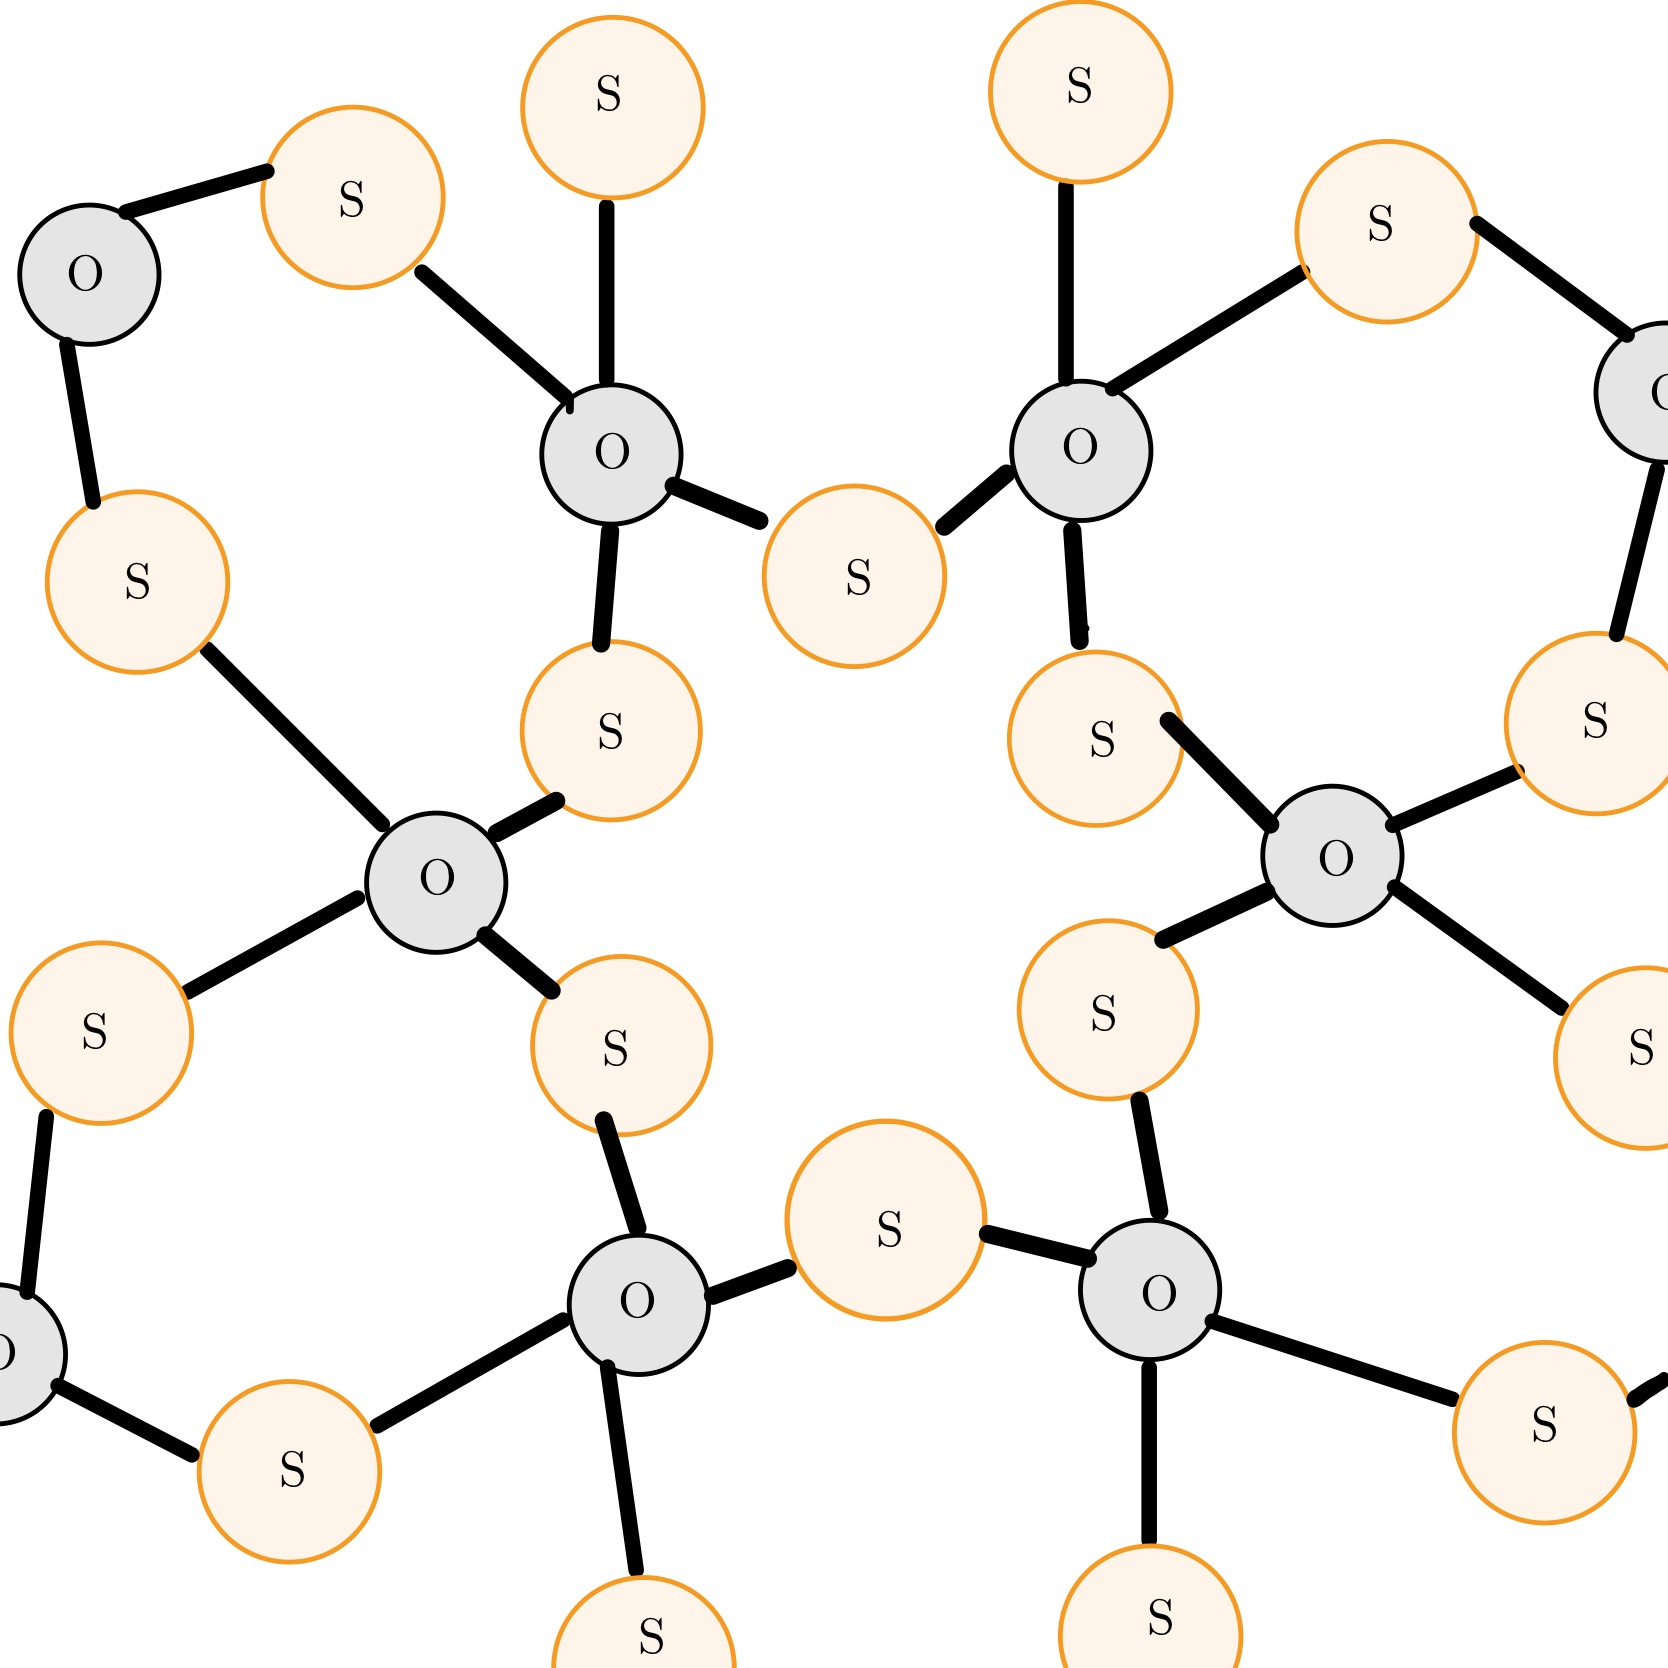
\includegraphics[width=\textwidth]{./Figure_1.jpg}
    \captionof{figure}{Structure of Quartz}
    \label{fig:Structue of Quartz}
\end{minipage}
\begin{minipage}{0.66\textwidth}
    To understand how a piezoelectric element works, one must have a look at the structure of a piezoelectric crystal. Most piezoelectric elements are made from quartz. Quartz is a material composed of silicon-dioxide whose structure can be seen in Figure \ref{fig:Structue of Quartz}. It is made of silicone and oxygen atoms arranged in a hexagonal shape. The silicone atoms are charged positively and the oxygen atoms negatively as the oxygen atom has a higher electronegativity.\cite{Mould2019}\\
\end{minipage}
\begin{minipage}{0.33\textwidth}
    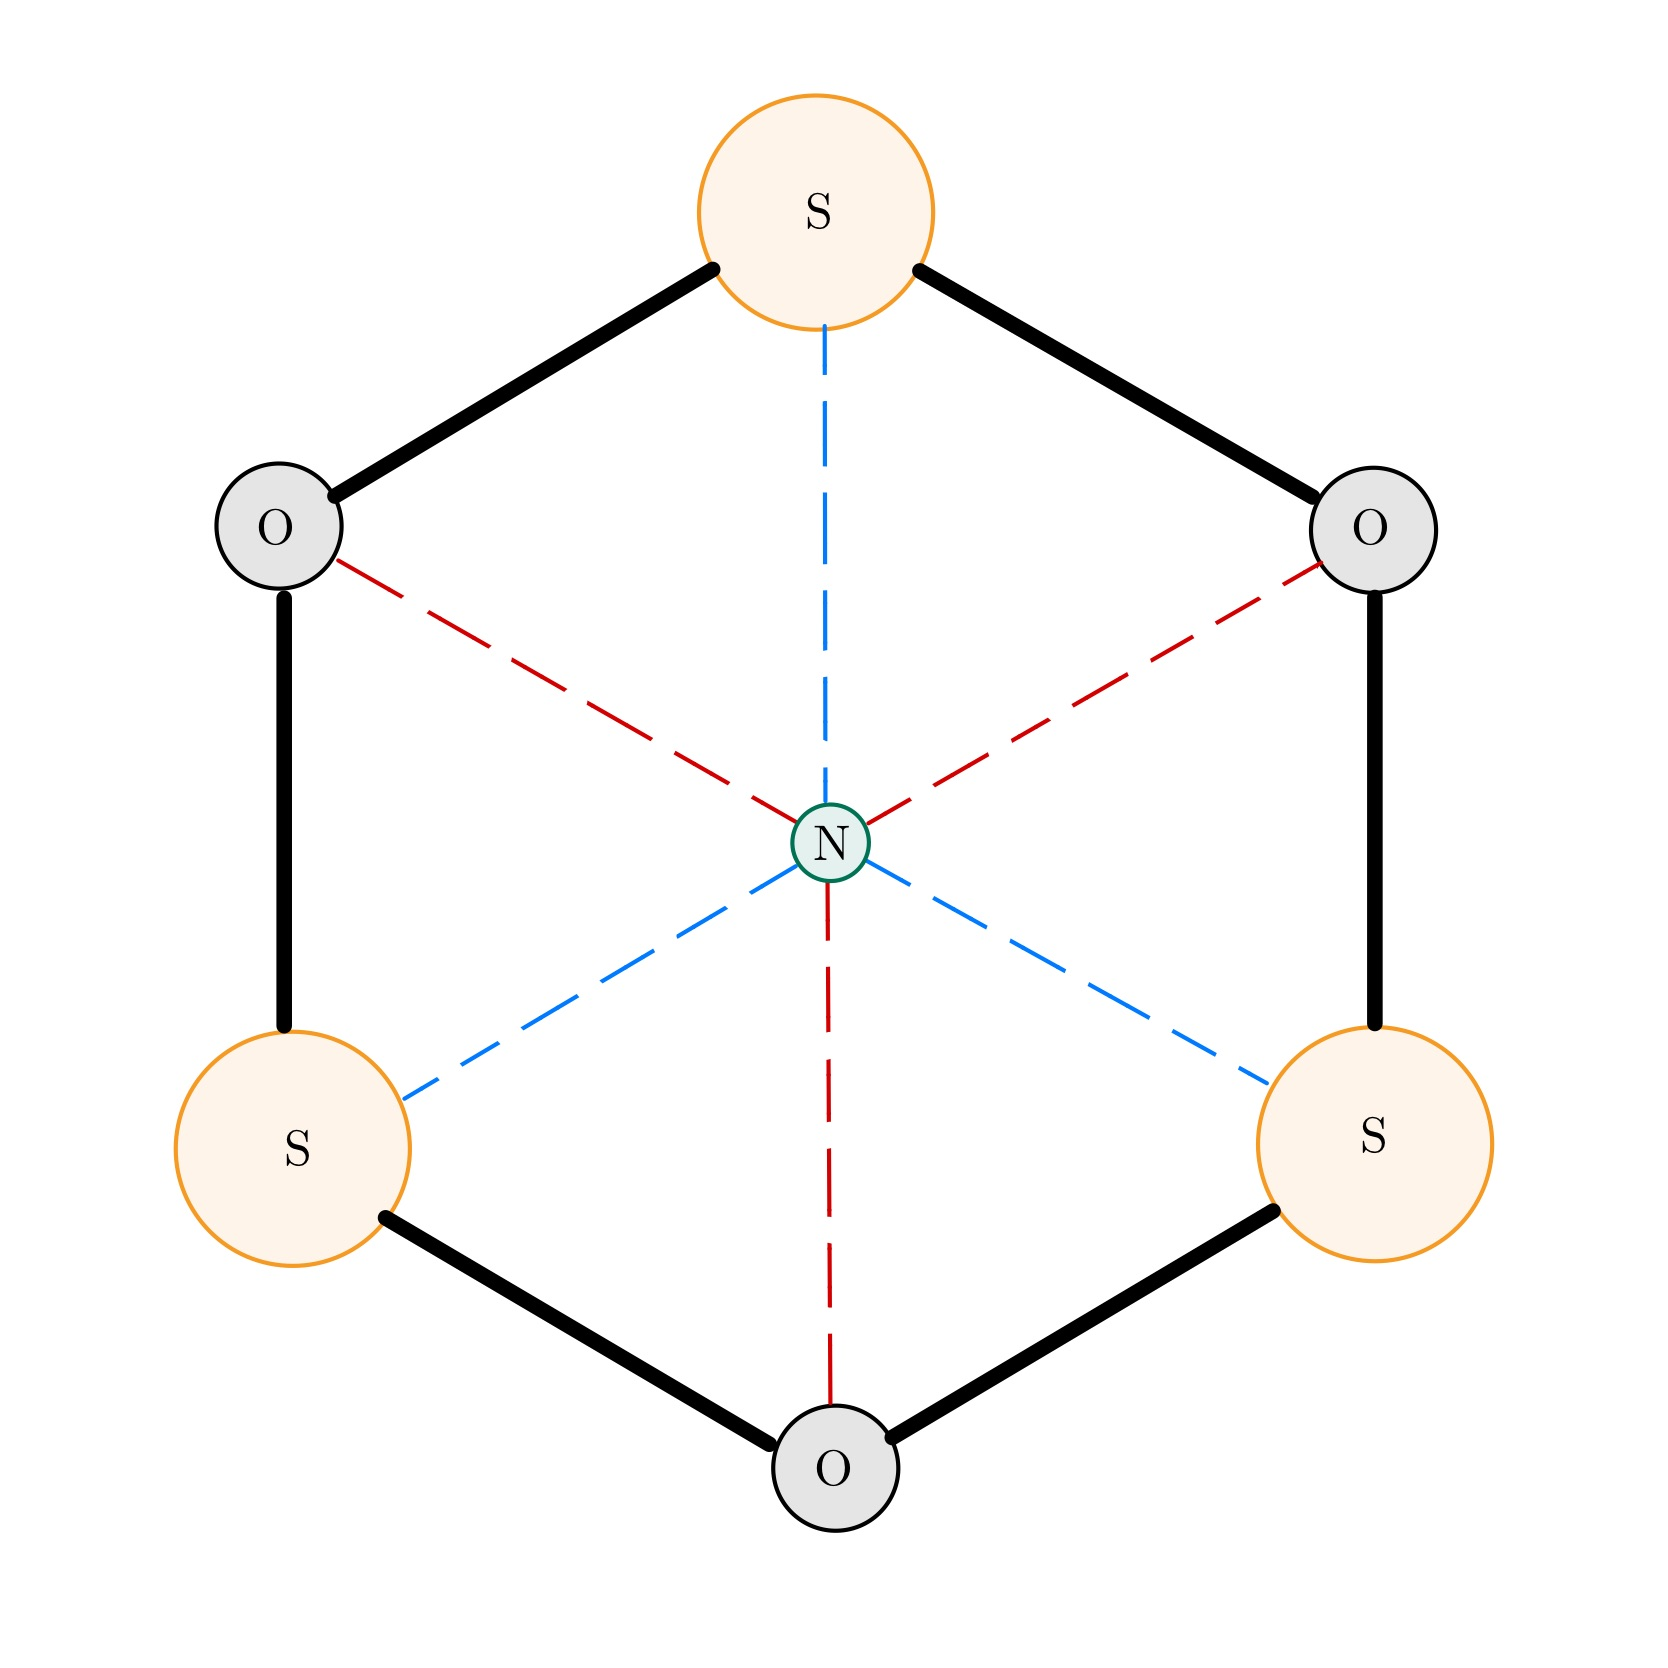
\includegraphics[width=\textwidth]{./Figure_2.jpg}
    \captionof{figure}{Quartzcell without any influence}
    \label{fig:Quartzcell without any influence}
\end{minipage}
\begin{minipage}{0.66\textwidth}
    In the beginning the average position of the charges overlap with each other which is visible in Figure \ref{fig:Quartzcell without any influence}. This means that no electromagnetic field is formed and thus no electric charge flows. However, when mechanical stress is applied onto the crystal the structure is changed.\cite{Mould2019}\\
\end{minipage}
\begin{minipage}{0.33\textwidth}
    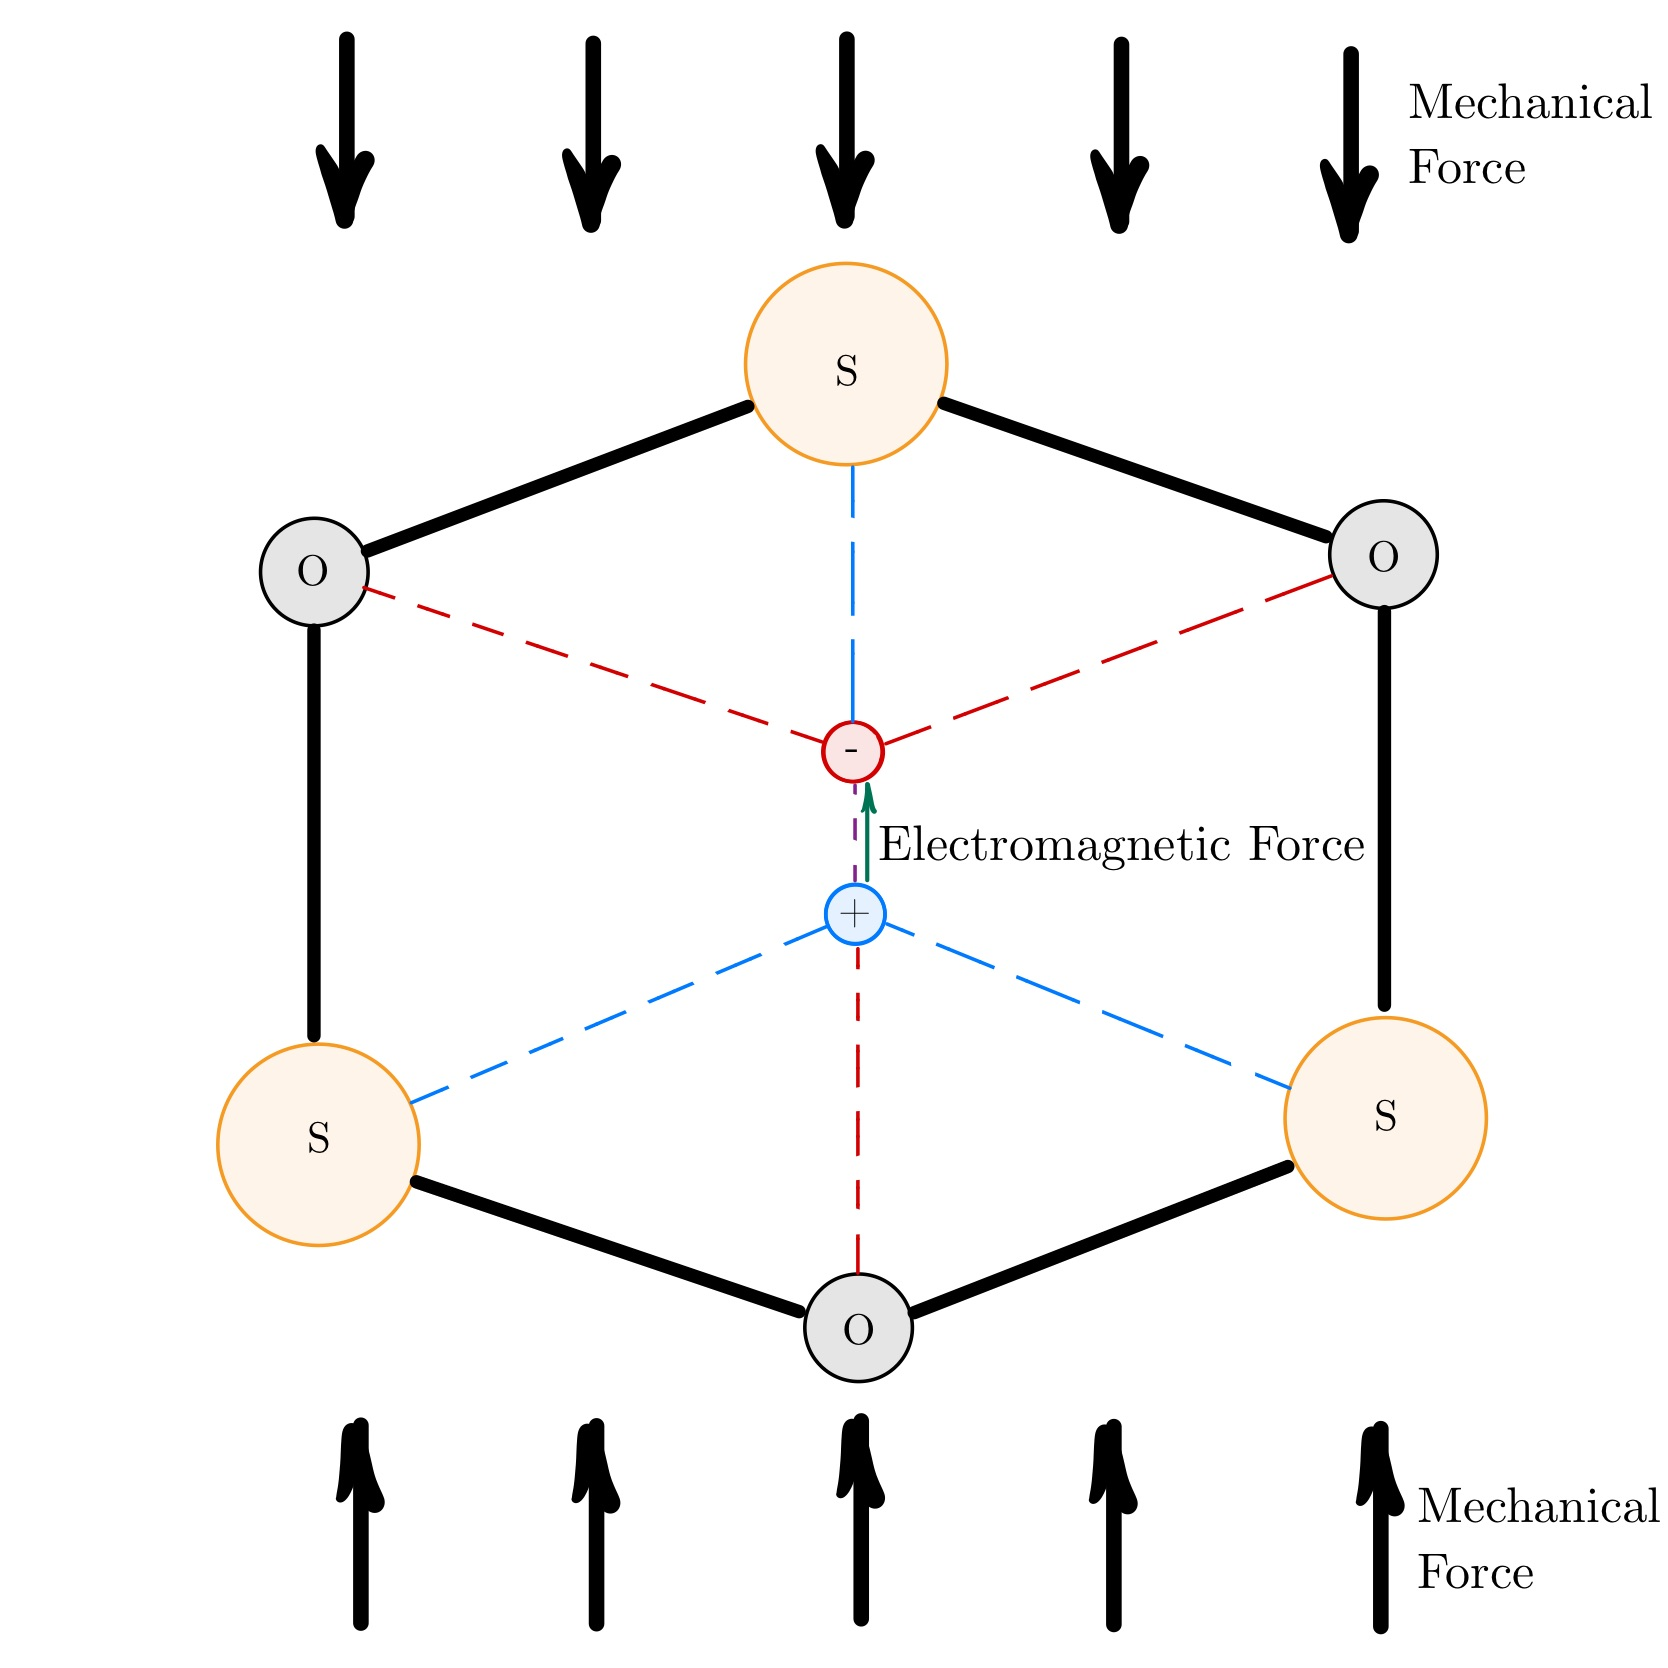
\includegraphics[width=\textwidth]{./Figure_3.jpg}
    \captionof{figure}{Quartzcell compressed}
    \label{fig:Quartzcell compressed}
\end{minipage}
\begin{minipage}{0.66\textwidth}
Mechanical stress can be either in the form of compression or expansion. In case of compression, the average position of the negative charge is moved upwards and the average position of the positive charge is moved downwards (Figure \ref{fig:Quartzcell compressed}) and vice versa when expanded.\cite{Mould2019}\\
\end{minipage}

\vspace{0.5cm}
\noindent In either way, a current can now flow as a positive face and a negative face is created. If a load such as a small LED is connected to the faces, the LED would blink. It is important to note is that the load must be connected correctly. The anode and cathode differ depending on the type of mechanical stress.\\
\begin{minipage}{0.33\textwidth}
    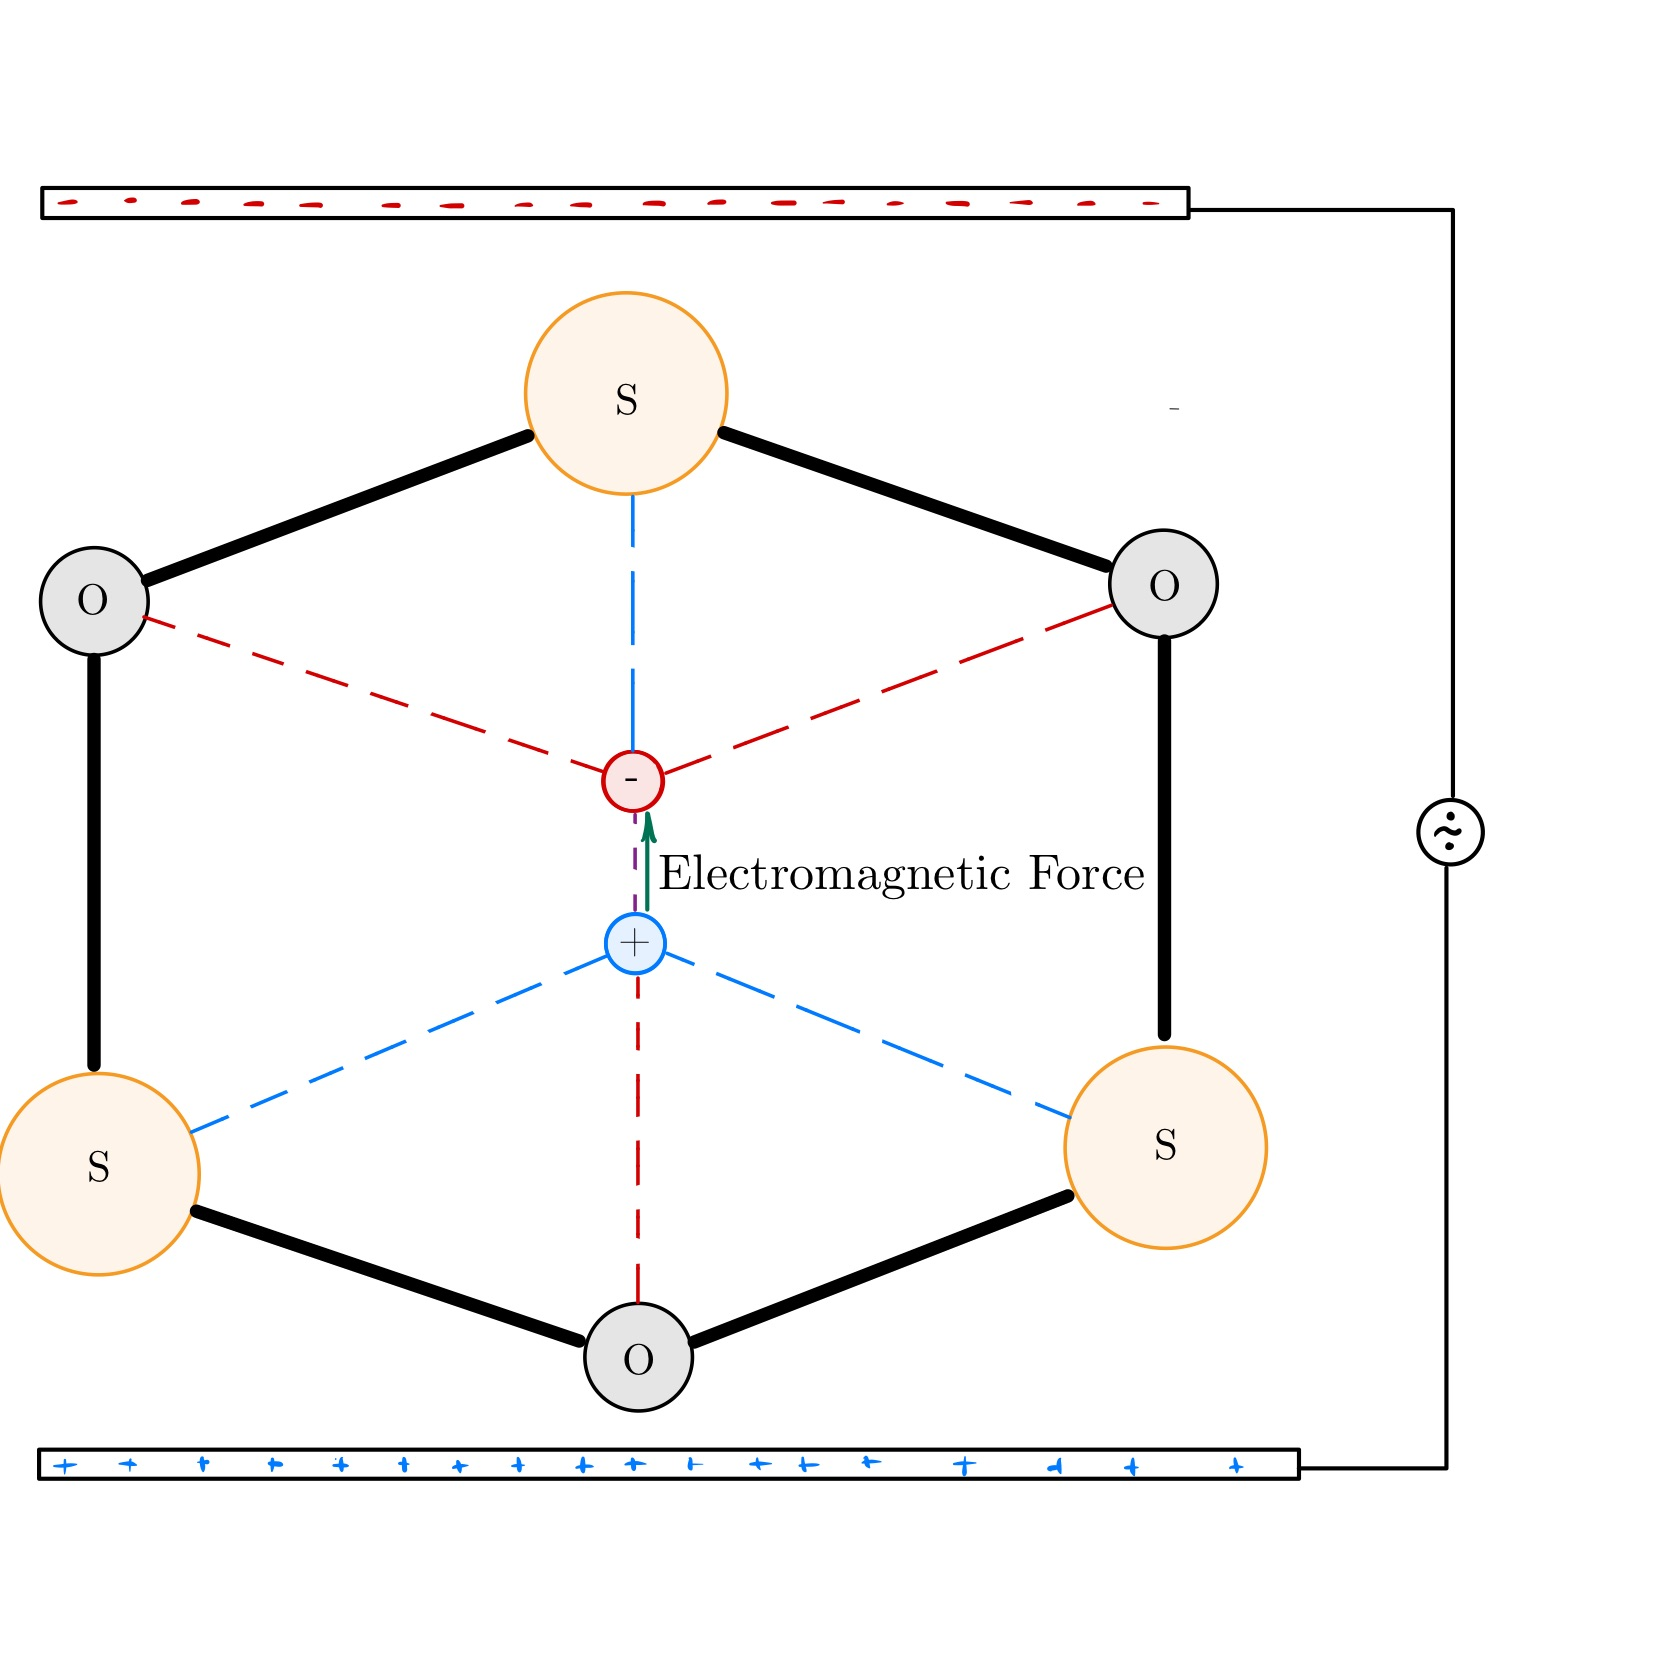
\includegraphics[width=\textwidth]{./Figure_4.jpg}
    \captionof{figure}{Quartzcell charged with a voltage}
    \label{fig:Quartzcell charged with a voltage}
\end{minipage}
\begin{minipage}{0.66\textwidth}
    Besides the mechanical stress, a voltage can be applied onto the crystal. This is refered to as the reciprocal piezoelectric effect. When the cathode and anode are positioned like in  Figure \ref{fig:Quartzcell charged with a voltage} the crystal will be compressed since the anode repels the negatively charged oxygen and the cathode repels the positively charged silicone and vice versa.\cite{Elprocus2023}\\
\end{minipage}
\\
 
\subsection{Formula}

To have a comparison with the measured voltage, the voltage output has to be calculated. The formula for the voltage output of a piezoelectric element can be calculated by simplifying the voltage output of a capacitor since the piezoelectric element is a capacitor.\cite{F3lixTutorial2023}\\
Before going through the process of simplifying the formula, two piezoelectric constants must be defined. There are many, however, only the electromechanical coupling factor and the piezoelectric voltage constant will be defined as only these constants will be used. The electromechanical coupling factor $d$ is defined as the effectiveness with which a piezoelectric element converts mechanical energy into electrical energy and vice versa. The piezoelectric voltage constant $g$ is defined as the electric field generated by a piezoelectric element per unit stress applied. The constants differ depending on the direction of mechanical stress or the electrical field.\cite{F3lixTutorial2023}\\
\begin{minipage}{0.33\textwidth}
    \vspace{0.5cm}
    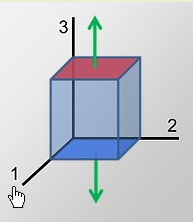
\includegraphics[width=\textwidth]{./Figure_5.jpg}
    \captionof{figure}{Expansion Mode of the Piezoelectric Element \cite{F3lixTutorial2023}}
    \label{fig:Expansion Mode of the Piezoelectric Element}
\end{minipage}
\begin{minipage}{0.66\textwidth}
    The constants are marked with numbers. These numbers correspond to the direction of mechanical stress and the polarization which is depicted in Table \ref{Tab:Piezoelectric Constants} and Figure \ref{fig:Expansion Mode of the Piezoelectric Element}. In our case $g_{33}$ and $d_{33}$ will be used since the force acting on the crystal is from direction 3 and the polarization occurs in direction 3.\cite{F3lixTutorial2023}\\ 
\end{minipage}
\begin{minipage}{0.5\textwidth}
    \center
        \begin{tabular}{|c|c|c|c|}
            \hline
            & PZT-5H & PZT-5A & PZT-5J \\
            \hline
            \hline
            $d_{31}$ & -320 & -190 & -270 \\
            \hline
            $d_{33}$ & 650 & 390 & 485 \\
            \hline
            $d_{15}$ & 1000 & 460 & 850 \\
            \hline
            $g_{31}$ & -9.5 & -11.3 & -11.5 \\
            \hline
            $g_{33}$ & 19.0 & 23.2 & 21.3 \\
            \hline
            $g_{15}$ & 35.3 & 32.4 & 32.6 \\
            \hline
        \end{tabular}
        \captionof{table}{Piezoelectric Constants \cite{Carter2023}}
        \label{Tab:Piezoelectric Constants}
\end{minipage}
\begin{minipage}{0.5\textwidth}
    From Table \ref{Tab:Piezoelectric Constants}, one can see that the constant also depends on the type of piezoelectric material. There are three types of piezoelectric materials which are commonly used. The piezoelectric material used in this experiment is of type PZT-5J since the material was made from ceramic and the cathode was made from silver. This ensures that the piezoelectric element performs well under the specific stress and voltage. Depending on the direction, the type of piezo is chosen to maximise the energy outcome. However, most piezos are of type PZT-5J since they are considered to be an allrounder for any case of stress or voltage. \cite{Carter2023}\\
\end{minipage}
Since the piezoelectric element is a capacitor, the formula $U=\frac{Q}{C}$ can be used where $U$ is the voltage, $Q$ is the charge and $C$ is the capacity. From there the formula $\epsilon \cdot \frac{A}{t}$ is inserted where $\epsilon$ is the permitivity, $A$ is the surface area where the mechanical stress is applied on and $t$ is the thickness of the piezoelectric element. Furthermore, the formula $d \cdot F$ can be inserted for $Q$ where $F$ is the force applied onto the piezoelectric element and $d$ is the effeciveness with wwhich a piezoelectric element converts mechanical energy into electrical energy and vice versa. Once all equations are inserted, $U=\frac{d \cdot F \cdot t}{\epsilon \cdot A}$ where $\frac{d}{\epsilon}$ can be replaced with $g$. This results in the formula $U = g \cdot \frac{F \cdot t}{A}$ for the Voltage output of the piezoelectric element. \cite{F3lixTutorial2023}
$$
U = \frac{Q}{C} \quad \text{ where } C = \epsilon \cdot \frac{A}{t} \text{ and } Q = d \cdot F
$$
$$
U = \frac{d \cdot F \cdot t}{\epsilon \cdot A} \text{ where } g = \frac{d}{\epsilon}
$$
$$
U = g \cdot \frac{F \cdot t}{A}
$$
For the energy emitted by the piezoelectric element, on can use the formula for the energy of a spring since the compression and expansion is similar to a spring. Hence, the formula $E = \frac 1 2 \cdot F \cdot x$ applies where $E$ is the energy, $F$ is the force applied onto the piezoelectric element, and $x$ is the displacement of the element. Since $x$ is not known, it can be replaced by $\frac{F}{k}$ where $k$ is the sping constant of the piezoelectric element. This leads the formula $E = \frac{1}{2} \cdot F \cdot \frac F k$ for the energy outputted by the piezoelectric element.
$$
E = \frac{1}{2} \cdot F \cdot x \text{ where } x = \frac{F}{k}
$$
$$
E = \frac{1}{2} \cdot F \cdot \frac{F}{k}
$$